\documentclass[12pt]{standalone}
\usepackage[version=3]{mhchem}
\usepackage{tikz}     % draw stuff
\usepackage{pgfplots} % plot stuff
\pgfplotsset{compat=1.10} % avoid warnings

% Software titles
\newcommand{\ML}{\textsc{Matlab}}
\newcommand{\MLS}{\textsc{Matlab}/Simulink}

% Math tools
\newcommand{\dif}{\mathop{}\!\mathrm{d}}
\newcommand{\Dif}{\mathop{}\!\mathrm{D}}

\newcommand\pd[3][]{\frac{\partial^{#1}#2}{\partial#3^{#1}}}
\newcommand\tpd[3][]{\tfrac{\partial^{#1}#2}{\partial#3^{#1}}}
\newcommand\dpd[3][]{\dfrac{\partial^{#1}#2}{\partial#3^{#1}}}

\newcommand{\md}[6]{\frac{\partial^{#2}#1}{\partial#3^{#4}\partial#5^{#6}}}
\newcommand{\tmd}[6]{\tfrac{\partial^{#2}#1}{\partial#3^{#4}\partial#5^{#6}}}
\newcommand{\dmd}[6]{\dfrac{\partial^{#2}#1}{\partial#3^{#4}\partial#5^{#6}}}

\newcommand{\od}[3][]{\frac{\dif^{#1}#2}{\dif#3^{#1}}}
\newcommand{\tod}[3][]{\tfrac{\dif^{#1}#2}{\dif#3^{#1}}}
\newcommand{\dod}[3][]{\dfrac{\dif^{#1}#2}{\dif#3^{#1}}}

% Colors
\definecolor{notes}  {cmyk}{0.35,0.95,1.00,0.25}
\definecolor{string} {cmyk}{1.00,0.00,0.92,0.51}
\definecolor{comment}{gray}{0.3}

% Notes
\newcommand{\note}[1]{\marginpar{\SingleSpacing\flushleft\tiny\sffamily\color{notes}#1}}
\newcommand{\todo}[1]{\note{PDG TODO: #1}}

% Thermodynamic terms
\newcommand{\process}[2]{process~#1--#2}
\newcommand{\Process}[2]{Process~#1--#2}
\newcommand{\state}[1]{state~#1}
\newcommand{\State}[1]{State~#1}
\newcommand{\tssymb}{$T\!$-$s$}
\newcommand{\CV}{\mathrm{CV}}
\newcommand{\RE}{\mathrm{Re}}
\newcommand{\MA}{\mathrm{Ma}}
\newcommand{\NTU}{\mathrm{NTU}}

% Inlets and outlets
\newcommand{\inl}{\text{i}}
\newcommand{\out}{\text{o}}

% Velocities
\newcommand{\vel}{\mathscr{V}}
\newcommand{\svel}{a}

% Nomenclature Units
\newcommand{\nomunit}[1]{\renewcommand{\nomentryend}{\hspace*{\fill}\si{#1}}} % for convenience and consistency
\usepackage[adobe-garamond]{mathdesign}
\usepackage[no-math]{fontspec}
\setmainfont[
  Ligatures=TeX,
  Kerning=Uppercase,
  BoldFont={AGaramondPro-Semibold},
  Numbers=Proportional,
]{Adobe Garamond Pro}
\setsansfont[Ligatures=TeX]{Myriad Pro}
\setmonofont{Source Code Pro}
\setmathrm{Adobe Garamond Pro}
%\usepackage{kpfonts} % choose fonts from main thesis
\usepackage{siunitx}
\sisetup{%
  number-math-rm = \ensuremath, 
  sticky-per,
}
\let\DeclareIPUnit\DeclareSIUnit
\let\IP\SI
\let\ip\si
\DeclareIPUnit\horsepower{hp}
\DeclareIPUnit\foot{ft}
\DeclareIPUnit\inch{in}
\DeclareIPUnit\psia{psia}
\DeclareIPUnit\psig{psig}
\DeclareIPUnit\psid{psid}
\DeclareIPUnit\fahrenheit{\degree F}
\DeclareIPUnit\rankine{R}
\DeclareIPUnit\revolution{rev} % choose units from main thesis

\pgfplotsset{%
  proc/.style={%
    black,
    line width=1.1pt,
    arrows=-latex
  },
  refr/.style={%
    gray
  },
  range frame/.style={%
    axis lines*=left,
    tick align=outside,
    axis line style={opacity=0},
    after end axis/.code={
      \draw ({rel axis cs:0,0}-|{axis cs:\pgfplotsdataxmin,0}) -- ({rel axis cs:0,0}-|{axis cs:\pgfplotsdataxmax,0});
      \draw ({rel axis cs:0,0}|-{axis cs:0,\pgfplotsdataymin}) -- ({rel axis cs:0,0}|-{axis cs:0,\pgfplotsdataymax});
    }
  },
  parity plot/.style={%
    width=3in,
    height=3in,
    axis equal,
    scale only axis,
  },
}

\tikzset{%
  stat/.style={%
    circle,
    draw,
    fill=white,
    inner sep=1pt,
    outer sep=5pt,
  }
}

\newcommand{\drawstate}[3]{%
  \draw[fill=white] (axis cs:#1) circle (2pt) node[stat,#2] {#3};
}


\usetikzlibrary{calc,shapes,arrows}

\tikzstyle{general} = [rectangle, draw, text width=5em, text centered, node distance=4em]
\tikzstyle{process} = [general]
\tikzstyle{inoutput} = [general,draw=none]
\tikzstyle{terminal} = [general, rounded corners=0.75em, minimum height=1.5em]
\tikzstyle{decision} = [general, diamond, inner sep=0pt, node distance=3cm]
\tikzstyle{line} = [draw, -latex]

\newcommand{\drawprocess}[3]{%
  \node [process, #1] (#2) {#3};
  \draw ($(#2.south west)+(0.4em,0)$) -- ($(#2.north west)+(0.4em,0)$);
  \draw ($(#2.south east)+(-0.4em,0)$) -- ($(#2.north east)+(-0.4em,0)$);
}

\newcommand{\inoutput}[3]{%
  \node[inoutput, #1] (#2) {#3};
  \draw ($(#2.south west)+(-0.4em,0)$) -- ($(#2.north west)+(0.4em,0)$) -- ($(#2.north east)+(0.4em,0)$) -- ($(#2.south east)+(-0.4em,0)$) -- cycle;
}

\begin{document}
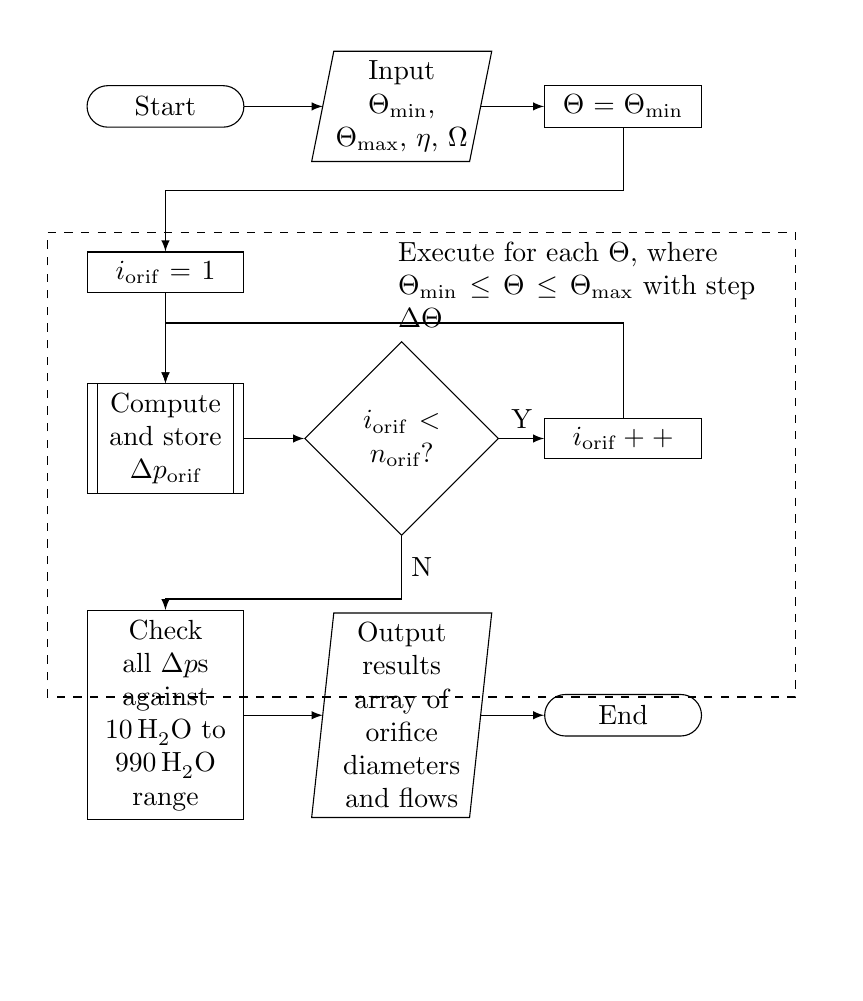
\begin{tikzpicture}[auto]
  % Place nodes
  \node[terminal] (start) {Start};
  \inoutput{right of=start,node distance=3cm}{input}{Input $\Theta_{\text{min}}$, $\Theta_{\text{max}}$, $\eta$, $\Omega$};
  \node[process,right of=input,node distance=8em] (init) {$\Theta = \Theta_{\text{min}}$};
  \node[process,below of=start,node distance=6em] (norif) {$i_{\text{orif}}=1$};
  \drawprocess{below of=norif, node distance=6em}{runmodel}{Compute and store $\Delta p_{\text{orif}}$}
  \node[decision,right of=runmodel] (ncheck) {$i_{\text{orif}} < n_{\text{orif}}$?};
  \node[process,right of=ncheck,node distance=8em] (increment) {$i_{\text{orif}}++$};
  \node[process,below of=runmodel,node distance=10em] (checkp) {Check all $\Delta p$s against \SIrange{10}{990}{\inch\ce{H2O}} range};
  \inoutput{below of=ncheck,node distance=10em}{output}{Output results array of orifice diameters and flows}
  \node[terminal,below of=increment,node distance=10em] (end) {End};
  
  \path[line] (start.east)--(input.west);
  \path[line] (input.east)--(init.west);
  \path[line] (init.south) -- ++(0,-0.8) -| (norif.north);
  \path[line] (norif.south)--(runmodel.north);
  \path[line] (runmodel.east)--(ncheck.west);
  \path[line] (ncheck.east)--(increment.west) node[midway] {Y};
  \path[line] (increment.north) -- ++(0,1.2) -| (runmodel.north);
  \path[line] (ncheck.south) -- ++(0,-0.8) node[midway] {N} -| (checkp.north);
  \path[line] (checkp.east)--(output.west);
  \path[line] (output.east)--(end.west);
  \draw[dashed] (-1.5,-7.5) rectangle (8,-1.6);
  
  \node[anchor=north east, text width=14em] at (8,-1.6) {Execute for each $\Theta$, where $\Theta_{\text{min}} \leq \Theta \leq \Theta_{\text{max}}$ with step $\Delta \Theta$};
  
  \path (-1.75,-11) rectangle (8.5,1);
\end{tikzpicture}
\end{document}
